% =====================================================================
%  Supplementary Information for the Wuhan-Shanghai optical-clock comparison
%  (paper/rev2/supplementary.tex -- standalone document)
%
%  Companion document to main.tex. All numbers are macros generated by
%  tools/build_numbers.py; see generated/numbers_manifest.json for
%  provenance. Do not edit numbers by hand.
%
%  Compile:  pdflatex supplementary.tex && pdflatex supplementary.tex
% =====================================================================
\documentclass[11pt,a4paper]{article}

\usepackage[T1]{fontenc}
\usepackage[utf8]{inputenc}
\usepackage{amsmath}
\usepackage{amssymb}
\usepackage{graphicx}
\usepackage{booktabs}
\usepackage{geometry}
\usepackage[hidelinks]{hyperref}

\usepackage{siunitx}
\sisetup{detect-all,separate-uncertainty=true,group-digits=all,group-minimum-digits=4}

\geometry{margin=2.5cm}

% Generated by tools/build_numbers.py -- do not edit by hand.
% Provenance for every macro: generated/numbers_manifest.json.

\newcommand{\Rheadline}{1.207\thinspace507\thinspace039\thinspace343\thinspace337\thinspace720\thinspace1}
\newcommand{\RbayesFull}{1.2075070393433377201344585656369188179292550569336320493567391993015505600807042}
\newcommand{\RwlsFull}{1.2075070393433377201300363286261481205336963758023772463919635856100035202592917}
\newcommand{\RmpFull}{1.2075070393433377201300363286261481205336963758023772463919635856100035202592917}
\newcommand{\RwlsHead}{1.207\thinspace507\thinspace039\thinspace343\thinspace337\thinspace720\thinspace1}
\newcommand{\RmpHead}{1.207\thinspace507\thinspace039\thinspace343\thinspace337\thinspace720\thinspace1}
\newcommand{\RbayesHead}{1.207\thinspace507\thinspace039\thinspace343\thinspace337\thinspace720\thinspace1}
\newcommand{\RwlsHeadT}{1.207\thinspace507\thinspace039\thinspace343\thinspace337\thinspace720\thinspace130}
\newcommand{\RmpHeadT}{1.207\thinspace507\thinspace039\thinspace343\thinspace337\thinspace720\thinspace130}
\newcommand{\RbayesHeadT}{1.207\thinspace507\thinspace039\thinspace343\thinspace337\thinspace720\thinspace134}
\newcommand{\RwlsRawT}{1.207507039343337720130}
\newcommand{\RmpRawT}{1.207507039343337720130}
\newcommand{\RbayesRawT}{1.207507039343337720134}
\newcommand{\uStatE}{1.139}
\newcommand{\uStatShort}{1.14}
\newcommand{\uWlsE}{1.128}
\newcommand{\uMpE}{1.128}
\newcommand{\uBirgeE}{0.725}
\newcommand{\chiSq}{6.18}
\newcommand{\chiRed}{0.412}
\newcommand{\dofV}{15}
\newcommand{\pChi}{\ensuremath{9.8\times10^{-1}}}
\newcommand{\birgeRatio}{0.642}
\newcommand{\xiMpE}{0.00}
\newcommand{\xiBayesE}{0.14}
\newcommand{\muBayesE}{\ensuremath{-0.676}}
\newcommand{\sensRwlsHead}{1.207\thinspace507\thinspace039\thinspace343\thinspace337\thinspace720\thinspace4}
\newcommand{\sensChiRed}{0.51}
\newcommand{\dSegNineWls}{\ensuremath{+0.29\times10^{-18}}}
\newcommand{\tidalChiRaw}{0.41}
\newcommand{\tidalChiTheory}{0.57}
\newcommand{\tidalChiEmp}{0.54}
\newcommand{\tidalShiftEmpE}{0.85}
\newcommand{\tidalShiftAltE}{0.21}
\newcommand{\tidalChiAlt}{0.50}
\newcommand{\nSeg}{16}
\newcommand{\nSegAll}{17}
\newcommand{\nSamples}{986\thinspace416}
\newcommand{\nSamplesAll}{1\thinspace008\thinspace912}
\newcommand{\nHours}{274}
\newcommand{\nHoursAll}{280}
\newcommand{\nSegNine}{22496}
\newcommand{\nModelLimited}{5}
\newcommand{\modelLimitedGroups}{\ensuremath{2,\ 6,\ 7,\ 12,\ 16}}
\newcommand{\uSrE}{0.92}
\newcommand{\uYbE}{1.3}
\newcommand{\uLinkE}{0.1}
\newcommand{\uCombE}{0.1}
\newcommand{\uTidalE}{0.85}
\newcommand{\dWVal}{280.042}
\newcommand{\dWUnc}{0.085}
\newcommand{\dWAlt}{280.60}
\newcommand{\dWAltUnc}{2.558}
\newcommand{\refNistV}{1.207\thinspace507\thinspace039\thinspace343\thinspace337\thinspace723\thinspace0}
\newcommand{\refNistU}{37}
\newcommand{\refNistE}{3.7}
\newcommand{\refEuV}{1.207\thinspace507\thinspace039\thinspace343\thinspace337\thinspace718}
\newcommand{\refEuU}{32}
\newcommand{\refEuE}{3.2}
\newcommand{\fibreKm}{1\thinspace350}
\newcommand{\roundKm}{2\thinspace700}
\newcommand{\siteKm}{700}
\newcommand{\levelKm}{1\thinspace113}
\newcommand{\nDays}{58}
\newcommand{\nStages}{3}
\newcommand{\refSameCampusU}{\ensuremath{3.2\times10^{-18}}}
\newcommand{\refSameCampusKm}{3.6}
\newcommand{\refEuBestU}{\ensuremath{7.7\times10^{-18}}}
\newcommand{\refPtbTransportableU}{\ensuremath{4.3\times10^{-18}}}
\newcommand{\baconE}{\ensuremath{8\times10^{-18}}}
\newcommand{\nemitzU}{\ensuremath{5\times10^{-17}}}
\newcommand{\refVlbiKm}{9\thinspace000}
\newcommand{\refLisdatKm}{1\thinspace415}
\newcommand{\fRepMHz}{200}
\newcommand{\fFifteenTHz}{193.3992}
\newcommand{\deltaGV}{\ensuremath{-3.116\times10^{-15}}}
\newcommand{\uSubsystemBound}{\ensuremath{1\times10^{-19}}}
\newcommand{\levelMm}{0.255}
\newcommand{\refThreshold}{\ensuremath{5\times10^{-18}}}
\newcommand{\selfEvalBound}{\ensuremath{2\times10^{-18}}}
\newcommand{\refLisdatU}{\ensuremath{5\times10^{-17}}}
\newcommand{\euNClocks}{7}
\newcommand{\euNInstitutes}{4}
\newcommand{\lindvallNClocks}{10}
\newcommand{\lindvallNCountries}{6}
\newcommand{\lindvallNRatios}{38}
\newcommand{\schioppoKm}{\ensuremath{2\,220}}
\newcommand{\chenKm}{\ensuremath{2\,067}}
\newcommand{\claimDate}{October 2026}
\newcommand{\uStaticE}{0.946}
\newcommand{\uTotalE}{2.34}
\newcommand{\uTotalShort}{2.3}
\newcommand{\RheadlineUnc}{28}
\newcommand{\dVsNistE}{\ensuremath{-2.87\times10^{-18}}}
\newcommand{\dVsEuE}{\ensuremath{+2.13\times10^{-18}}}


\newcommand{\dff}{\Delta f/f}
\newcommand{\dW}{\Delta W}

\title{Supplementary Information: \siteKm-km intercity Yb/Sr optical
clock comparison at \uTotalShort$\times10^{-18}$}

\author{xxxxx}

\date{}

\begin{document}
\maketitle

\section{Per-segment data}

\begin{table}[h]
  \centering
  \caption{Per-segment data of the 16 segments analyzed in this work.
  Ratio deviations $y_i = R_i/R_1 - 1$ are relative to the first
  segment, with $R_1 = \RsegOne$. $u(y_i)$ is the statistical
  uncertainty of the segment ratio;
  ``Fit'' is \emph{est.} for segments whose stability fit lies in the
  white-frequency-noise band and \emph{lim.} for model-limited fits.}
  \label{tab:segments}
  % Generated by tools/build_numbers.py -- do not edit by hand.
\begin{tabular}{rrrrl}
\toprule
Group & $n_{\rm valid}$ & $y_i$ ($10^{-18}$) & $u(y_i)$ ($10^{-18}$) & Fit \\
\midrule
1 & 68\,009 & +0.00 & 4.245 & est. \\
2 & 29\,481 & -3.36 & 3.017 & lim. \\
3 & 42\,891 & +2.00 & 5.880 & est. \\
4 & 64\,280 & -4.61 & 3.674 & est. \\
5 & 19\,532 & -3.38 & 15.250 & est. \\
6 & 52\,140 & -1.15 & 2.230 & lim. \\
7 & 39\,526 & +5.31 & 3.476 & lim. \\
8 & 43\,565 & +0.97 & 9.860 & est. \\
10 & 57\,938 & -0.76 & 5.003 & est. \\
11 & 35\,824 & +2.61 & 5.976 & est. \\
12 & 40\,346 & +0.73 & 4.843 & lim. \\
13 & 152\,994 & -3.09 & 4.019 & est. \\
14 & 68\,618 & +1.97 & 6.254 & est. \\
15 & 57\,649 & -0.25 & 4.028 & est. \\
16 & 147\,640 & -0.77 & 1.809 & lim. \\
17 & 65\,983 & -0.89 & 8.813 & est. \\
\bottomrule
\end{tabular}

\end{table}

\begin{figure}[h]
  \centering
  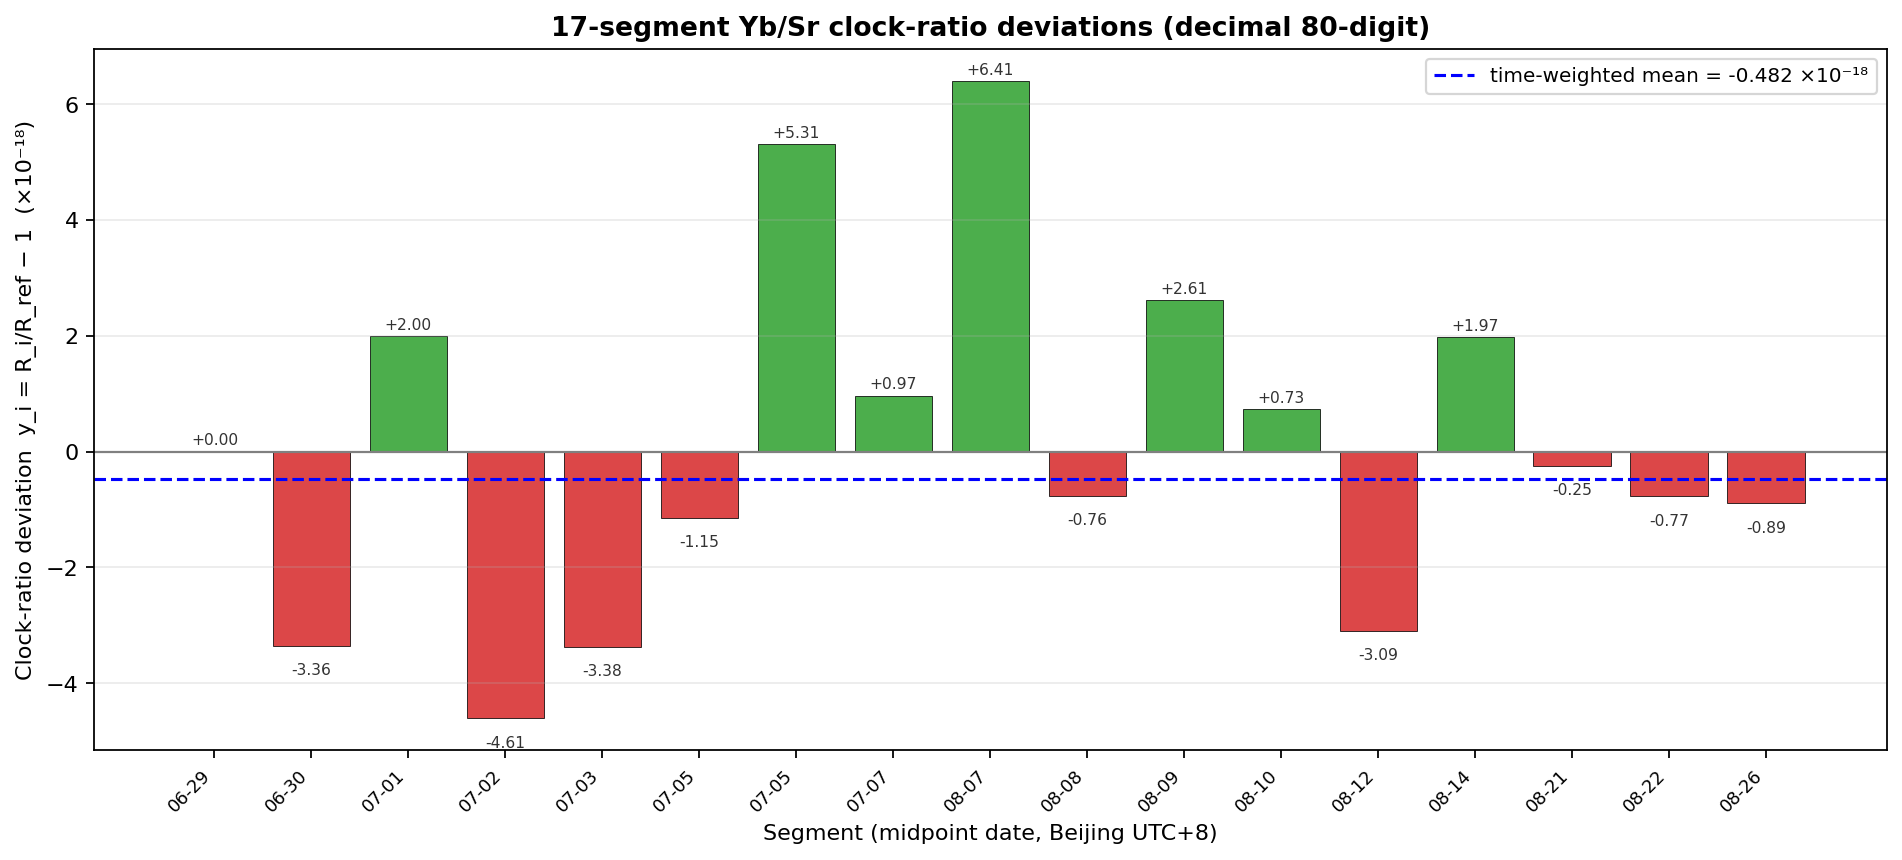
\includegraphics[width=0.9\linewidth]{figs/figSI_ratio_segments.png}
  \caption{Per-segment ratio deviations $y_i$ ($\times10^{-18}$,
  relative to the first segment) with their statistical
  uncertainties, over the campaign. No systematic drift is
  visible; the numerical values are in Table~\ref{tab:segments}.}
  \label{fig:ratio-segments}
\end{figure}

\begin{table}[h]
  \centering
  \caption{Intermediate quantities of the per-segment ratio
  inversion: the retained sample count $n_{\rm valid}$, the
  segment-mean beat deviation $\overline{\delta b}$ and the Sr
  systematic shift $a$ entering the Dr formula, and the resulting
  ratio $R_i$ (24 digits shown; full precision in the frozen result
  layer).}
  \label{tab:ratio-intermediates}
  % Generated by tools/build_numbers.py -- do not edit by hand.
\begin{tabular}{rrrrr}
\toprule
Segment & $n_{\rm valid}$ & $\overline{\delta b}$ (Hz) & $a$ & $R_i$ \\
\midrule
1 & 68\,009 & -0.025397 & -1.720e-16 & 1.2075070393433377209510 \\
2 & 29\,481 & -0.024746 & -1.720e-16 & 1.2075070393433377168993 \\
3 & 42\,891 & -0.025789 & -1.720e-16 & 1.2075070393433377233626 \\
4 & 64\,280 & -0.024502 & -1.720e-16 & 1.2075070393433377153827 \\
5 & 19\,532 & -0.024747 & -1.720e-16 & 1.2075070393433377168737 \\
6 & 52\,140 & -0.025168 & -1.720e-16 & 1.2075070393433377195622 \\
7 & 39\,526 & -0.026376 & -1.718e-16 & 1.2075070393433377273671 \\
8 & 43\,565 & -0.025530 & -1.717e-16 & 1.2075070393433377221180 \\
9 & 57\,938 & +0.009546 & +7.906e-18 & 1.2075070393433377200284 \\
10 & 35\,824 & +0.008892 & +7.906e-18 & 1.2075070393433377241064 \\
11 & 40\,346 & +0.009259 & +7.917e-18 & 1.2075070393433377218315 \\
12 & 152\,994 & +0.009998 & +7.917e-18 & 1.2075070393433377172166 \\
13 & 68\,618 & +0.009019 & +7.917e-18 & 1.2075070393433377233303 \\
14 & 57\,649 & +0.009448 & +7.917e-18 & 1.2075070393433377206498 \\
15 & 147\,640 & +0.009549 & +7.917e-18 & 1.2075070393433377200195 \\
16 & 65\,983 & +0.009573 & +7.917e-18 & 1.2075070393433377198709 \\
\bottomrule
\end{tabular}

\end{table}

\begin{table}[h]
  \centering
  \caption{Leave-one-out sensitivity of the ratio combination. Each
  row excludes one of the 16 segments and recomputes the combination
  from the remaining segments. The center values are stable at the
  $10^{-18}$ level under any single exclusion.}
  \label{tab:loo}
  % Generated by tools/build_numbers.py -- do not edit by hand.
\begin{tabular}{rSSSS}
\toprule
Excluded segment & {$R_{\rm wls}$} & {$\chi^2_{\rm red}$} & {$u_{\rm wls}$ ($10^{-18}$)} & {$R_{\rm bayes}$} \\
\midrule
1 & 1.2075070393433377204 & 0.542 & 1.136 & 1.2075070393433377204 \\
2 & 1.2075070393433377208 & 0.474 & 1.164 & 1.2075070393433377208 \\
3 & 1.2075070393433377203 & 0.531 & 1.123 & 1.2075070393433377204 \\
4 & 1.2075070393433377208 & 0.451 & 1.145 & 1.2075070393433377208 \\
5 & 1.2075070393433377204 & 0.540 & 1.111 & 1.2075070393433377204 \\
6 & 1.2075070393433377206 & 0.535 & 1.217 & 1.2075070393433377206 \\
7 & 1.2075070393433377199 & 0.347 & 1.150 & 1.2075070393433377199 \\
8 & 1.2075070393433377204 & 0.542 & 1.114 & 1.2075070393433377204 \\
9 & 1.2075070393433377204 & 0.543 & 1.128 & 1.2075070393433377204 \\
10 & 1.2075070393433377203 & 0.525 & 1.122 & 1.2075070393433377203 \\
11 & 1.2075070393433377204 & 0.539 & 1.130 & 1.2075070393433377204 \\
12 & 1.2075070393433377206 & 0.512 & 1.139 & 1.2075070393433377206 \\
13 & 1.2075070393433377204 & 0.533 & 1.121 & 1.2075070393433377204 \\
14 & 1.2075070393433377204 & 0.543 & 1.139 & 1.2075070393433377204 \\
15 & 1.2075070393433377206 & 0.540 & 1.287 & 1.2075070393433377206 \\
16 & 1.2075070393433377204 & 0.543 & 1.115 & 1.2075070393433377204 \\
\bottomrule
\end{tabular}

\end{table}

\begin{table}[h]
  \centering
  \caption{Per-segment selection diagnostics. Counts at each stage of
  the data processing chain: the observation window, the excluded
  intervals, the jump-filtered record, the endpoint-trimmed samples
  and the retained count.}
  \label{tab:selection}
  % Generated by tools/build_numbers.py -- do not edit by hand.
\begin{tabular}{rrrrrr}
\toprule
Segment & window & excluded & jump-filtered & trimmed & retained \\
\midrule
1 & 68\,011 & 0 & 68\,011 & 2 & 68\,009 \\
2 & 29\,491 & 1 & 29\,488 & 4 & 29\,481 \\
3 & 42\,899 & 0 & 42\,896 & 3 & 42\,891 \\
4 & 64\,286 & 1 & 64\,283 & 0 & 64\,280 \\
5 & 19\,538 & 0 & 19\,538 & 6 & 19\,532 \\
6 & 52\,154 & 0 & 52\,154 & 14 & 52\,140 \\
7 & 39\,600 & 1 & 39\,599 & 73 & 39\,526 \\
8 & 43\,607 & 0 & 43\,606 & 37 & 43\,565 \\
9 & 57\,959 & 0 & 57\,957 & 16 & 57\,938 \\
10 & 35\,841 & 0 & 35\,839 & 12 & 35\,824 \\
11 & 40\,374 & 0 & 40\,374 & 28 & 40\,346 \\
12 & 153\,000 & 0 & 153\,000 & 6 & 152\,994 \\
13 & 68\,624 & 0 & 68\,621 & 0 & 68\,618 \\
14 & 57\,653 & 0 & 57\,653 & 4 & 57\,649 \\
15 & 147\,650 & 0 & 147\,650 & 10 & 147\,640 \\
16 & 66\,013 & 0 & 66\,013 & 30 & 65\,983 \\
\bottomrule
\end{tabular}

\end{table}

\section{Within-segment tidal correlation analysis}

As an independent quantitative check of the tide-model corrections
shown in the spliced stability figure of the Methods, each segment's
1200-s demeaned beat waveform was fitted against the 1-s tidal
template, $\mathrm{beat} = A\cdot\mathrm{tide}$, with the template
sign corrected for the beat polarity so that a positive amplitude
corresponds to the expected response $A = +1$; amplitudes,
Pearson $r$ and $p$ values were inferred from non-overlapping 1200-s
windows only. No single segment reaches a significant correlation on
its own: the per-segment fits scatter around zero with uncertainties
comparable to the template variation. Across the \nSeg~segments
entering the ratio combination, however, the sign of the correlation
is positive in \tidalNegSeg~of the \nSeg~segments for both tide
models, and the precision-weighted response amplitudes are
$\tidalAmpOldE$ (ETideLoad4.5) and $\tidalAmpNewE$
(DE421+FES2022), both differing from zero at more than $5\sigma$ but
falling short of the expected $+1$ and differing from each other.
This is the same conclusion as the spliced stability record: the
observed tidal coupling is real but smaller than any single template
predicts, so the tidal term is carried as an uncertainty.

\begin{table}[h]
  \centering
  \caption{Per-segment 1200-s-windowed tidal-correlation fits
  (ETideLoad4.5 template). $A$ and $u_A$ are the fitted amplitude and
  its uncertainty, $r$ the Pearson correlation, all from
  non-overlapping 1200-s windows; the sign convention has the
  expected response at $A=+1$. The combined, precision-weighted
  amplitude is $\tidalAmpOldE$ ($\tidalSigmaOldE\sigma$ from zero),
  with the sign of the correlation positive in \tidalNegSeg~of the
  \nSeg~segments; the DE421+FES2022 template gives $\tidalAmpNewE$
  ($\tidalSigmaNewE\sigma$) with the same sign count.}
  \label{tab:correlation}
  % Generated by tools/build_numbers.py -- do not edit by hand.
\begin{tabular}{rrrrr}
\toprule
Segment & hours & $A$ & $u_A$ & $r$ \\
\midrule
1 & 18.9 & -0.91 & 0.36 & -0.30 \\
2 & 8.2 & -0.54 & 0.52 & -0.45 \\
3 & 11.9 & -1.00 & 0.35 & -0.44 \\
4 & 17.9 & -0.28 & 0.35 & -0.06 \\
5 & 5.4 & -1.85 & 1.05 & -0.45 \\
6 & 14.5 & -0.16 & 0.37 & +0.13 \\
7 & 11.0 & -0.61 & 0.65 & +0.08 \\
8 & 12.1 & +0.38 & 0.94 & -0.03 \\
9 & 16.1 & -0.90 & 0.61 & -0.18 \\
10 & 10.0 & -0.86 & 2.18 & -0.08 \\
11 & 11.2 & -0.22 & 0.58 & -0.15 \\
12 & 42.5 & -0.32 & 0.32 & -0.04 \\
13 & 19.1 & -1.08 & 0.28 & -0.51 \\
14 & 16.0 & +0.15 & 0.87 & +0.08 \\
15 & 41.0 & -0.04 & 0.54 & +0.02 \\
16 & 18.3 & -0.12 & 0.51 & -0.05 \\
\bottomrule
\end{tabular}

\end{table}

\begin{figure}[h]
  \centering
  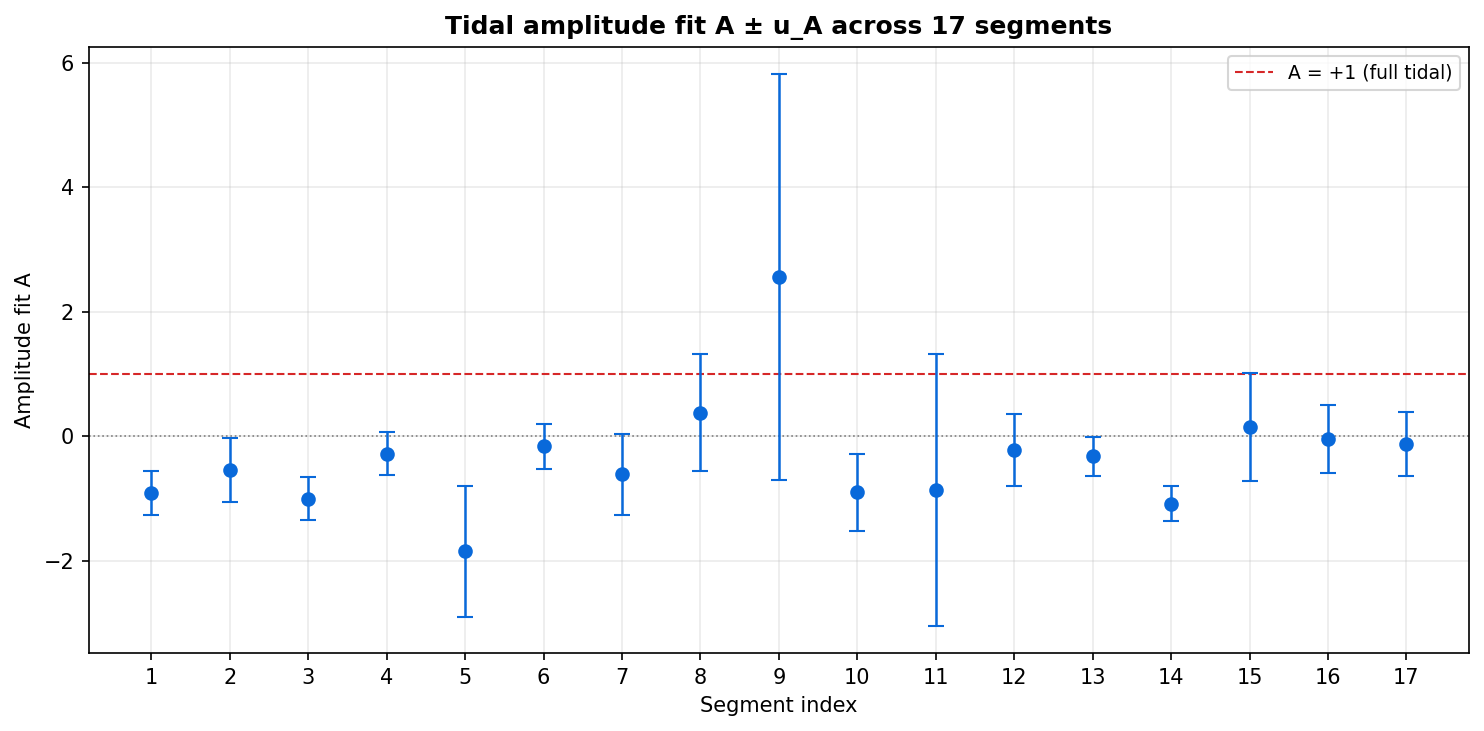
\includegraphics[width=0.95\linewidth]{figs/figSI_batch_forest.png}
  \caption{Forest plot of the per-segment tidal response amplitudes
  $A$ and their uncertainties (ETideLoad4.5 template, 1200-s
  windowed, sign convention with the expected response at $A=+1$).
  The gray band marks the precision-weighted combination
  $\tidalAmpOldE$; no single segment is individually significant,
  while the combination differs from zero at
  $\tidalSigmaOldE\sigma$.}
  \label{fig:forest}
\end{figure}

Environmental checks accompany this analysis. Surface air
temperature records at the three cities along the link show a clear
diurnal cycle (peak-to-peak about 4.6--5.6\,$^\circ$C), but the
diurnal components of the out-of-loop reference, the out-of-loop
signal and the fiber-link beat are each far below their respective
measurement noise, and the beat reflects the frequency difference
between the two clocks, so the temperature cycle is not detectable in
the record. Co-seismic displacement from the regional seismicity
during the campaign is estimated from the earthquake moments to be
at most $6\times10^{-20}$ in differential fractional frequency, two
orders below the statistical uncertainty, so it cannot drive the
tidal-period correlation.

\begin{table}[h]
  \centering
  \caption{Spliced concatenated stability of the \nSeg~segments at
  representative averaging times: the overlapping Allan deviation
  $\sigma_y(\tau)$ of the spliced record for the raw series, the two
  theoretical tide corrections ($A=+1$, ETideLoad4.5 and
  DE421+FES2022), the two empirical corrections ($A=+0.54$), and the
  removed correction terms themselves. The full $\tau$ grid and the
  pair counts are in the archived data.}
  \label{tab:spliced}
  % Generated by tools/build_numbers.py -- do not edit by hand.
\begin{tabular}{rSSSSSSS}
\toprule
{$\tau$ (s)} & {raw} & {ETL theory} & {ETL empir.} & {D+F theory} & {D+F empir.} & {corr.\ ETL} & {corr.\ D+F} \\
\midrule
1,200 & 1.53e-17 & 1.53e-17 & 1.53e-17 & 1.53e-17 & 1.53e-17 & 6.78e-19 & 5.26e-19 \\
3,600 & 8.20e-18 & 8.12e-18 & 8.12e-18 & 8.12e-18 & 8.14e-18 & 1.60e-18 & 1.25e-18 \\
7,200 & 5.95e-18 & 5.73e-18 & 5.67e-18 & 5.63e-18 & 5.68e-18 & 2.73e-18 & 2.14e-18 \\
16,384 & 4.71e-18 & 5.04e-18 & 4.45e-18 & 4.33e-18 & 4.23e-18 & 4.10e-18 & 3.13e-18 \\
43,200 & 2.85e-18 & 3.58e-18 & 3.06e-18 & 3.14e-18 & 2.92e-18 & 2.28e-18 & 1.46e-18 \\
86,400 & 2.01e-18 & 2.36e-18 & 2.14e-18 & 2.15e-18 & 2.05e-18 & 1.10e-18 & 7.96e-19 \\
172,800 & 1.37e-18 & 1.20e-18 & 1.22e-18 & 1.33e-18 & 1.31e-18 & 7.58e-19 & 6.24e-19 \\
400,000 & 8.57e-19 & 8.95e-19 & 8.10e-19 & 8.51e-19 & 8.03e-19 & 6.80e-19 & 5.80e-19 \\
\bottomrule
\end{tabular}

\end{table}

\begin{table}[h]
  \centering
  \caption{Three-scenario tidal combination summary (16 segments):
  the reduced chi-square and Birge ratio of the segment combination,
  the Bayesian excess scatter $\xi$, and the segment-to-segment
  spread $\sigma(y_i)$, for the raw record and for the two fixed
  correction amplitudes. Both corrections degrade the combination
  statistics.}
  \label{tab:tidal-synthesis}
  % Generated by tools/build_numbers.py -- do not edit by hand.
\begin{tabular}{lrrrr}
\toprule
Scenario & $\chi^2_{\rm red}$ & Birge & $\xi_{\rm Bayes}$ ($10^{-18}$) & $\sigma(y_i)$ ($10^{-18}$) \\
\midrule
raw ($A=0$) & 0.412 & 0.642 & 0.14 & 2.581 \\
theory ($A=+1$) & 0.573 & 0.757 & 0.16 & 2.473 \\
empirical ($A=+0.54$) & 0.537 & 0.733 & 0.15 & 2.334 \\
\bottomrule
\end{tabular}

\end{table}

\section{Frequency-chain relations and the ratio inversion}
\label{sec:freq-chain}

The two clock transitions are bridged to the \qty{1550}{nm} telecom
carrier through fixed factor-of-two relations. On the Shanghai side
the Sr \qty{698}{nm} transition is doubled to \qty{1397}{nm}; on the
Wuhan side the Yb \qty{578}{nm} transition is doubled to
\qty{1156}{nm}. Both ends are phase-locked to independent optical
frequency combs whose repetition rate is
$f_{\mathrm{rep}} = \fRepMHz$\,MHz, derived from a
\qty{10}{MHz} reference divided by 20.

The recorded observable is the out-of-loop beat $b$ between the
received carrier and the local Yb-referenced comb, sampled every
second. The ratio inversion uses the fixed chain constants
\begin{center}
\begin{tabular}{llll}
\toprule
Constant & Value & Meaning \\
\midrule
$N_{1156}$ & 1,295,739 & Yb 1156 nm comb count \\
$N_{1397}$ & 858,456 & Sr 1397 nm comb count \\
$N_{1550}$ & 773,598 & 1550 nm link count (Shanghai end) \\
$N_{1550}^{\rm WH}$ & 966,996 & 1550 nm link count (Wuhan end) \\
$f_{\mathrm{ref}}$ & \qty{10}{MHz} & comb repetition base \\
$\mathrm{div}_{20}$ & 20 & divider ($f_{\mathrm{rep}} = 200$ MHz) \\
\bottomrule
\end{tabular}
\end{center}

The beat is converted to fractional units with the transfer frequency
$f_{1550} = \fFifteenTHz$\,THz ($= N_{1550}^{\rm WH}\,f_{\mathrm{rep}}$).
The segment-mean beat deviation $\overline{\delta b}$ enters the
Sr/Yb ratio through
\[
\mathrm{Dr} = \frac{c_{1156}}{N_{1156}}\,
\frac{\overline{\delta b}}{f_{\mathrm{ref}}\,\mathrm{div}_{20}}
\bigg/ \left[
\frac{c_{1397}}{N_{1397}}
\left(N_{1550} + \frac{7}{25} + \frac{1}{25}\right)
\right],
\]
where $c_{1156} = (1+b_{\rm Yb})/2$ with $b_{\rm Yb} = -1.7\times10^{-18}$
(Yb-side fixed shift) and $c_{1397} = (1+a)/2$, with $a$ collecting the
five Sr systematic components listed below. The segment ratio is
\[
\mathrm{Sr/Yb} = \mathrm{ratio}_{\rm base} + \mathrm{Dr},
\qquad
\mathrm{ratio}_{\rm base} =
\frac{c_{1156}}{N_{1156}}\,
\frac{N_{1550}^{\rm WH} + \frac{26}{20} + \frac{m}{f_{\mathrm{ref}}\,\mathrm{div}_{20}}}
{\frac{c_{1397}}{N_{1397}}\left(N_{1550} + \frac{8}{25}\right)},
\]
where $m$ is the campaign-global median of the plausible beat samples.
The static gravitational-redshift correction is applied as a
multiplicative factor,
\[
(\mathrm{Yb/Sr})_{\rm corr} = (\mathrm{Yb/Sr})_{\rm raw}\,(1+\delta_g),
\qquad \delta_g = \deltaGV .
\]
All ratio arithmetic is carried out in 80-digit decimal precision,
mirroring the campaign processing convention.

The Sr systematic shift $a$ is the sum of five components evaluated
per segment: lattice AC-Stark ($a_{\rm rou}$, about
$-2.3$ to $-3.5\times10^{-19}$), AC Stark ($a_{\rm AC}$, $+7.44$ or
$+8.93\times10^{-18}$ by campaign period), second-order Zeeman
($a_{\rm SM}$, the dominant term), air refractive index
($a_{\rm air} = -6.7\times10^{-19}$), and blackbody radiation
($a_{\rm BBR} = 0$). The full per-segment values are listed in
Table~\ref{tab:shift-components}; the fixed chain constants are given
above, and the Yb-side fixed shift is $b_{\rm Yb} = -1.7\times10^{-18}$
with the static gravitational correction
$\delta_g = \deltaGV$.

\begin{table}[h]
  \centering
  \caption{Per-segment Sr systematic-shift components ($a_{\rm rou}$,
  $a_{\rm AC}$, $a_{\rm SM}$, $a_{\rm air}$, $a_{\rm BBR}$) of the 16
  segments analyzed in this work, as recorded in the campaign
  parameter file; $a = a_{\rm rou} + a_{\rm AC} + a_{\rm SM} +
  a_{\rm air} + a_{\rm BBR}$ enters the ratio inversion.}
  \label{tab:shift-components}
  \input{generated/shift_components_table}
\end{table}

\section{Statistical model and combination}

Each segment $i$ contributes a ratio estimate $R_i$ and a statistical
uncertainty $u_i$ obtained from the overlapping Allan deviation
$\sigma_y(\tau)$ of the beat fractional frequency, evaluated on a tau
grid of powers of two plus 600, 1200, 3600 and 7200\,s, limited to a
quarter of the longest gap-free run of the segment. $u_i$ adopts the
last computable point, $u_i = R_i\,\sigma_y(\tau_{\max})$, without
extrapolating the stability curve beyond the data; the log-log slope
of $\sigma_y(\tau)$ is retained as a white-frequency-noise diagnostic
only.

The choice of the last computable point is deliberate and
conservative. The beat record develops a low-frequency plateau for
$\tau \gtrsim 4096$\,s (a flicker-frequency-noise floor from the
clocks and the link, not the tides); fitting the white-frequency
slope and extrapolating it to the full segment duration would
systematically understate $u_i$ by 30--40\%, inflating the reduced
chi-square to about 4 and making the segments appear mutually
inconsistent. Adopting $\sigma_y$ at the largest computable $\tau$
instead keeps the statistical uncertainty honest at the expense of
being somewhat conservative: the resulting $\chi^2_{\rm red} = 0.41$
and Birge ratio 0.64 are below unity, indicating that the segments
are consistent with their (slightly conservative) uncertainties.
Segments whose log-log slope leaves the white-frequency-noise band
$[-0.65, -0.35]$ are flagged as model-limited but retained with their
measured uncertainties; they lie at the steep end of a continuous
slope distribution with no common campaign, weather or laboratory
condition.

The segments are combined under a random-effect model with common
excess scatter, $R_i \sim \mathcal{N}(\mu, u_i^2 + \xi^2)$. Three
estimators are evaluated:

\begin{itemize}
\item \emph{Weighted least squares} with inverse-variance weights
$w_i = 1/u_i^2$: $\hat\mu = \sum w_i R_i/\sum w_i$, with
$u_{\rm wls} = 1/\sqrt{\sum w_i}$. The reduced chi-square
$\chi^2_{\rm red} = \sum (R_i-\hat\mu)^2/u_i^2/(N-1)$ and the Birge
ratio $\sqrt{\chi^2_{\rm red}}$ quantify the segment agreement.

\item \emph{Mandel--Paule}: the same observation model with
$\xi$ chosen so that $\chi^2_{\rm red}(\xi) = 1$.

\item \emph{Bayesian random effect}: flat priors on $\mu$ and on
$\log\xi$, with the joint posterior marginalized numerically over a
40-decade $\log\xi$ grid (401 points, trapezoidal quadrature). The
grid span is expanded until the posterior mass at the edges falls
below 1\%. The posterior mean of $\mu$ and its posterior standard
deviation give the reported central value and statistical
uncertainty.
\end{itemize}

All three center values are reconstructed in decimal precision from
the segment-1 baseline, $R = R_1\,(1+\hat\mu/R_1)$, so that
differences at the $10^{-18}$ level are not lost in floating-point
arithmetic.

\section{Leveling details and national-standard comparison}

The first-order spirit leveling line runs about $\levelKm$\,km between
the Wuhan benchmark WS-03 and the Shanghai benchmark WS-01 through
Ezhou, Huangshi, Huanggang, Lu'an, Hefei, Wuhu, Guangde and Suzhou.
Digital levels with bar-code invar staffs were used, with sight
lengths not exceeding \qty{30}{m}; the line was observed in
\qtyrange{6}{8}{km} sections in both directions, each checked in the
field, and gravity was observed along the line at the leveling points
with two relative gravimeters. The per-kilometer accidental error is
$M_\Delta = \levelMm$\,mm\,km$^{-1}$. The most stringent first-order
requirements of the national standards of China (GB/T 12897--2006,
$M_\Delta \le 0.45$\,mm\,km$^{-1}$), the United States (FGCC 1984,
$0.5$\,mm\,km$^{-1/2}$), Germany (AdV FA-PN 2022, $0.4$\,mm) and
Czechia (\v{C}\'UZK 2015, $m_0 = 0.40$\,mm\,km$^{-1}$) are all
satisfied.

The independent GNSS-plus-geoid check used precise point positioning
for the ellipsoidal heights of the permanent marks, local leveling
for the vertical offsets to the clock reference surfaces, and the
EGM2008 geoid model for the conversion to geopotential, giving
$\dWAlt \pm \dWAltUnc~\mathrm{m^2\,s^{-2}}$, consistent with the
leveled value but about 30 times less precise, so it serves as a
consistency check rather than an independent calibration at the
reported accuracy.

\section{Tidal template construction and the two tide models}

The primary tide template is the solid Earth tide and ocean tide
loading displacement difference between the two sites, computed every
\qty{30}{s} with the public software ETideLoad4.5, which implements
the geophysical models and numerical standards of the IERS
Conventions (2010). The displacement difference is converted to an
equivalent geopotential difference with the local gravity
$g = 9.794$\,m\,s$^{-2}$ and then to a beat-frequency template
$h = f_{1550}\,\Delta W/c^2$ with the same $f_{1550}$ normalization as
the beat record; the direction convention is
$\Delta W = W(\mathrm{Wuhan}) - W(\mathrm{Shanghai})$.

The cross-check template computes the solid tide from the DE421
ephemerides (Earth--Sun--Moon positions) with Love numbers, and takes
the ocean-tide loading correction to the gravitational potential
directly from the FES2022 global ocean-tide model, on a \qty{90}{s}
Beijing-time grid. The two templates are independent realizations;
their mutual correlation over the campaign is $+0.88$, and their
segment-mean predictions differ in detail.

The historical response amplitude $A = +0.54$ used for the
fixed-amplitude combinations comes from the demeaned beat waveform of
an earlier analysis of the same campaign: the precision-weighted
amplitude of a 1200-s-windowed, demeaned fit of the beat against the
ETideLoad4.5 template was $+0.54$, with a standard uncertainty of
about $0.08$. As an independent consistency check, a grid scan of
fixed amplitudes $A_{\rm fix} \in \{-1.0, -0.54, -0.30, -0.20, 0,
+0.20, +0.54, +1.0\}$, applied to the within-segment residuals, finds
its residual-correlation zero crossing at $A_{\rm fix} \approx +0.54$,
matching the fitted value; the same analysis locates the dominant
coupling in the ocean-tide loading term, since the solid tide alone
gives a markedly weaker segment-mean correlation (see the main text).
The amplitude is carried as a fixed historical value rather than a
free parameter of this work.

\section{Transfer subsystems}

The fiber route is divided into spans of tens of kilometers, each
terminated by a relay station carrying a narrow-linewidth laser, an
erbium-doped fiber amplifier and a fiber-noise-cancellation loop; 21
independent relay stations carry 22 amplifiers in total. The link
extends the field-deployed cascade of a previous
\qty{2067}{km} demonstration, and its added instability is kept below
the clock noise for averaging times beyond $100$\,s. Both frequency
combs are self-referenced and phase-locked to their local clock
signal; all other frequencies in the chain derive from the two clock
transitions through the fixed factor-of-two relations of
Section~\ref{sec:freq-chain}, so the two clocks are the system's only
independent frequency sources. The fiber loop-back is monitored out
of loop throughout. The frequency-conversion stages each contribute
below $\uSubsystemBound$ to the uncertainty budget, from the
digitization error of the direct-digital-synthesis
frequency-reference settings; the budget carries them as
\qty{0.1e-18} upper bounds.

\end{document}
